% kapitel2.tex
\chapter{Grundlagen}
\label{chapter:grundlagen}

%%% Titel Grundlagen von Tomaten???

In diesem Kapitel werden die Grundlage bezüglich der Tomatepflanze sowie der verschiedenen Pflanzenkrankheiten behandelt. Der Abschnitt \ref{botanik} klärt zunächst auf, wie Tomaten grundsätzlich aufgebaut sind, welche Bedingungen sie für das Wachstum brauchen sowie die allgemeine wirtschaftliche Bedeutung ist. Im Abschnitt \ref{sec:Blattkrankheiten} werden vier Pflanzenkrankheiten vorgestellt, die die Blätter von Tomaten angreifen. 

\section{Botanik von Tomaten}
\label{botanik}

Die Tomate (lat. Solanum lycopersicum), die als Gemüsefrucht eingeordnet wird und in Europa als \glqq Liebesapfel\grqq~bekannt wurde, ist mit der Kartoffel verwandt\cite{nutzInDE}. Des Weiteren stammt sie von der Familie der Nachtschattengewächse (lat. Solanaceae) ab und lässt sich schwer von Obst abgrenzen, da sie als Obstmahlzeit, Rohkost oder gekocht verzehrt werden kann. Unter die Kategorie Gemüsefrucht zählen Früchte, die "[...] kaum süß schmecken, bisweilen unreif geerntet, herzhaft zubereitet und zum Teil ausschließlich gekocht gegessen werden", (\cite{nutzpflanzen}, S. 231). 


\subsection{Herkunft}

Die Herkunft der heutigen Kulturtomate ist zur Zeit unklar. Lediglich einige Herkunftsorten können laut dem Autor Körber-Grohne\cite{nutzInDE} in Frage kommen. Hierbei werden die nördlichen Gebiete von Südamerika sowie die Karibik genannt, die an unterschiedlichen Orten angesiedelt sind. Dort existieren vier Arten der Wildtomate mit roten Früchten:


\begin{itemize}
	\item \textbf{Kirschenförmige Wildtomate} (L. cerasiforme): Diese Sorte stammt aus Südamerika und verbreitete sich in den tropischen bzw. subtropischen Gebieten von Europa, Asien und Afrika. Daher ist diese Sorte am weitesten verbreitet. 
	
	\item \textbf{Johannisbeertomate} (L. pimpinellifolia): Diese Sorte ist durch die Größe der Frucht gekennzeichnet, da sie der Größe einer Johannisbeere entspricht.
	
	\item \textbf{Humboldts Wildtomate} (L. humboldtii): In den Flußniederungen und am Seeufer ist diese Sorte in Venezuela verbreitet. Des Weiteren sind die Früchte vier mal größer als die kirschförmige Wildtomate.
	
	\item \textbf{Wildtomate} (L. cheesmanii): Da diese Sorte auf den Galapagosinseln am Strand wächst, ist sie unempfindlich gegen das Meerwasser. Außerdem kann sie mit Meerwasser gegossen werden, wobei andere Wildtomatenarten davon einen Schaden erleiden können.  
	 
\end{itemize}

Eine weitere Herkunftsmöglichkeit könnte Mexiko sein. Stammend aus den Ländern Ecuador und Peru wurde die Tomate von den ortsansässigen Inkas nicht als Nahrungsmittel wertgeschätzt\cite{nutzpflanzen}. Erst nach der Ausbreitung der Pflanze als Unkraut nach Norden wurde diese durch die Hochkultur Mexikos gezüchtet. Im Tehuacan-Tal südlich von der Hauptstadt Mexikos wurden erste Tomatensamen gefunden. Diese befanden sich in Höhlenschichten, die aus dem Zeitabschnitt 200 v. Chr. und 700 n. Chr. gebildet wurden. Zu diesem Zeitraum hat die Hochkultur Ackerbau mit künstlichen Bewässerungsanlagen betrieben\cite{nutzInDE}. Nach der Entdeckung von Amerika im 15. Jahrhundert\cite{nutzInDE, nutzpflanzen} verbreitete sich die Tomate lediglich in Italien, weil andere europäische Länder diese nicht als Nahrungsmittel verwendet haben. Bis zum 19. Jahrhundert wurde die Tomate im restlichen Europa sowie Nordamerika aufgrund der Zugehörigkeit des Nachtschattengewächses als giftig angesehen. In Deutschland setze sich erst die Tomate in den 20er Jahren des 19. Jahrhunderts durch. Andere europäische Länder, zum Beispiel Frankreich, Österreich und Ungarn, verwendeten die Tomate aufgrund des wärmeren Klimas deutlich früher als Deutschland. Erst in der Zeit ab 1920 wurde die Tomate \glqq[...] die weltweit bedeutendste Salat- bzw. Gemüsepflanze.\grqq,(\cite{nutzpflanzen}, S. 232).


\subsection{Aufbau und Fortpflanzung}
% https://cms.uni-konstanz.de/fileadmin/biologie/ag-doerken/pdf/Morphologie/3_Bluete.pdf


Einjährige krautige Tomatenpflanzen wachsen bis zu einer Höhe von 1.5m und haben nacheinanderfolgende verzweigte Sprossglieder. An diesen sind gefiederte, große Blätter versehen (s. Abbildung \ref{tomaten_aufbau}). Am Ende eines Sprossglieds befindet sich ein Blütenstand in Form einer Wickel. Der Sprossaufbau wird von den Achselknospen weitergeführt. Des Weiteren führt das eintriebige Ausbrechen der Achselknospen zu größeren Früchten. Das männliche reproduktive Organ der Blüte ist das sogenannte Staubblatt. Auf diesen Staubblättern befinden sich die verwachsenen Staubbeutel (Antheren) sowie die Staubfäden (Filament)\cite{Bluete}. Die Borstenhaare sind mit den Antheren der gelben Blüte zu einem zylindrischen Hohlkörper zusammengeführt, um den oberständigen Fruchtknoten einzuwickeln (s. Abbildung \ref{tomaten_both} links). Durch die Vibration der bestäubenden Insekten, die hauptsächlich Hummeln sind, können Pollen in den Antherenkegel eindringen, um eine Befruchtung der Pflanze zu ermöglichen. Da die Pflanze selbstfertil ist, kann sie sich auch ohne die Hilfe von Hummeln fortpflanzen.   

\begin{wrapfigure}{r}{8cm}
	\centering
	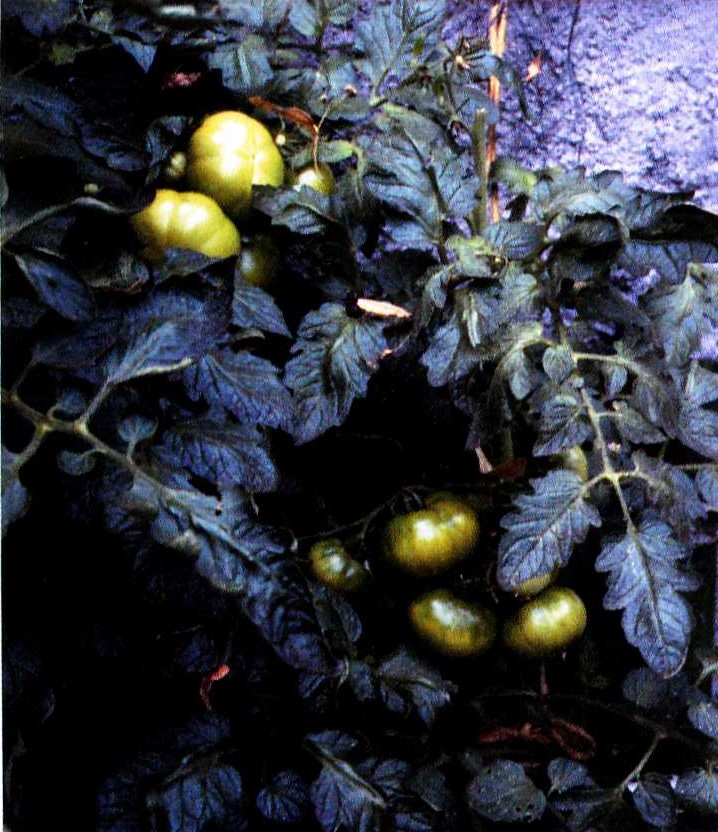
\includegraphics[width=0.4\textwidth]{bilder/nutzpfl_1.jpg}%
	\caption{Die Tomatenpflanze mit ihrem charakteristischen, verzweigten Aufbau\cite{nutzpflanzen}.}
	\label{tomaten_aufbau}
\end{wrapfigure}


Aus zwei verwachsenen Fruchtblättern, die aus mehreren Fächern bestehen und den Innenräumen entsprechen, setzt sich der Fruchtknoten zusammen \cite{Bluete, nutzpflanzen}. Dieser ist an einer zentralen Plazenta mit einigen Samenanlagen angebunden, die sich zu einem markreichen Gewebe im weiteren Verlauf entwickelt. In den Samenschalen befinden sich das sogenannte Myxotesta, welches sich als stark verschleimendes Zylinderepithel kennzeichnet (siehe Abbildung \ref{tomaten_both} rechts). Durch ein schleimiges Gewebe werden die Zwischenräume der Samen umschlossen, welches von der Plazenta abgesondert wird.


\begin{figure}[h!]
	\hfill
	\subfigure[]{
		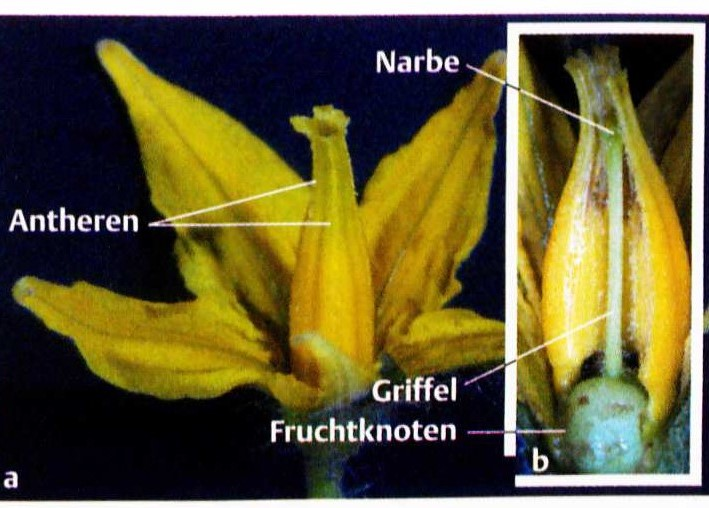
\includegraphics[width=0.45\textwidth]{bilder/nutzpfl_2a.jpg}}
	\hfill
	\subfigure[]{
		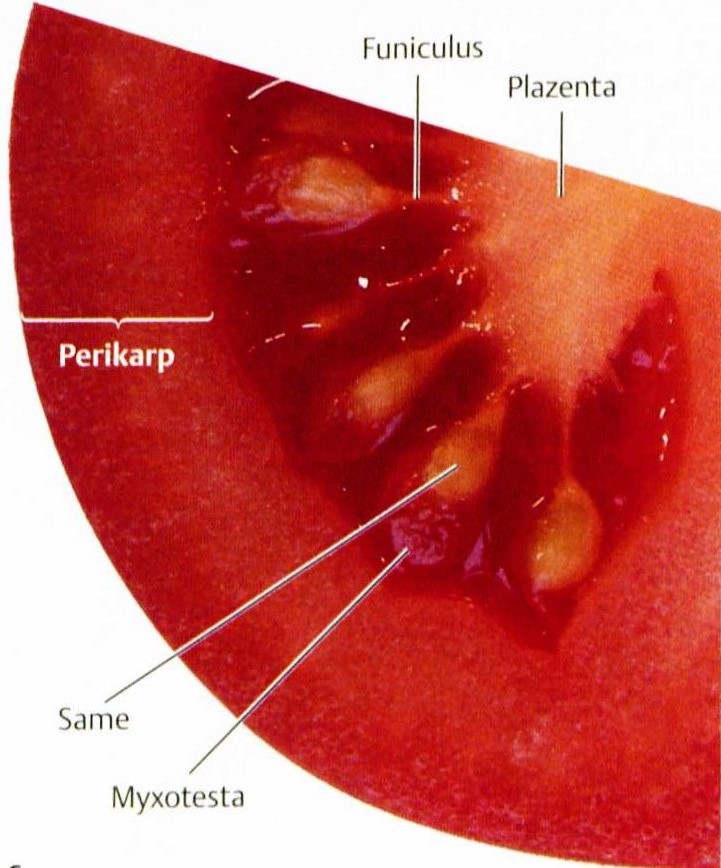
\includegraphics[width=0.45\textwidth]{bilder/nutzpfl_2b.jpg}}
	\hfill
	\caption{In der linken Darstellung wird die Blüte einer Tomate mit geöffneter Antherensäule veranschaulicht. Die rechte Abbildung zeigt einen Querschnitt der Frucht\cite{nutzpflanzen}.}
	\label{tomaten_both}
\end{figure}


\subsection{Anbau und Standortansprüche}



Aufgrund ihrer hohen Ansprüche und geringen Standfestigkeit benötigen Tomatenpflanzen, die an Pfählen oder hochgebundenen Seilen angebaut werden, bröckeligen, nährstoffreichen Boden. Da die Tomate ursprünglich aus den Tropen stammt\cite{nutzpflanzen}, können Kälteschäden auch bei Temperaturen über $0^\circ\text{C}$ auftreten. Deswegen werden Tomaten in Gewächshäusern gepflanzt, da sie dort nicht nur einen Schutz gegen die Kälte, sondern auch gegen Wind und Starkregen, erhalten. Außerdem werden für die Bestäubung der Pflanzen seit 1985 Hummeln (Bombus terrestris) ganzjährig eingesetzt. Hierfür werden diese speziell für den Tomatenanbau in Gewächshäusern gezüchtet.

\subsection{Wirtschaftliche Bedeutung}
%TODO: Quelle
%http://appsso.eurostat.ec.europa.eu/nui/submitViewTableAction.do einbauen

In diesem Abschnitt wird die wirtschaftliche Bedeutung von Tomaten betrachtet. Zunächst ist die Frage interessant, in welchen Mengen überhaupt in Deutschland Gemüse verzehrt wird. Anschließend werden die Erntemengen der europäischen Länder betrachtet.

\paragraph{Konsum von Tomaten}
~\newline

Der Verbrauch an Gemüse ist dank des statistischen Bundesamts\cite{bundesamt} klar dokumentiert. Die Abbildung \ref{pro_kopf_konsum} veranschaulicht in einem kleinen Ausschnitt den Pro-Kopf-Konsum in dem Zeitraum zwischen 2015 bis 2018 in Deutschland. Für vollständige Daten wird auf die Quelle verwiesen.

\begin{figure}[h!]
	\centering
	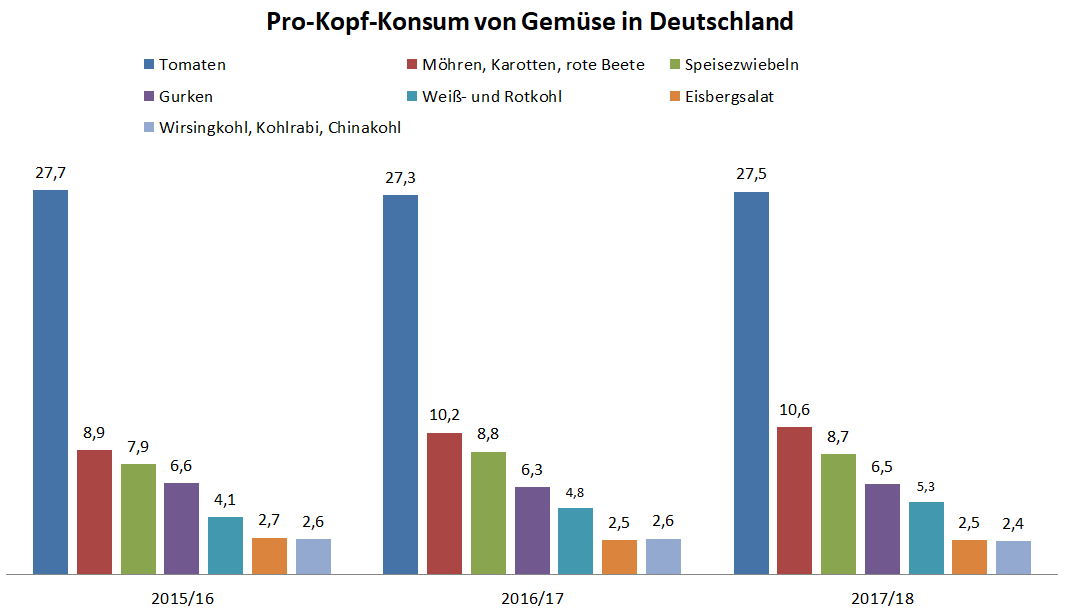
\includegraphics[width=\textwidth]{bilder/pro_kopf_konsum.PNG}
	\caption{Darstellung des Pro-Kopf-Konsums von Gemüse im Zeitraum 2015 - 2018\cite{bundesamt} (eigene Darstellung).}
	\label{pro_kopf_konsum}
\end{figure}

Auf der x-Achse sind einige Gemüsesorten als unterschiedlich gefärbte Säule aufgelistet. Auf der y-Achse befindet sich der Pro-Kopf-Konsum in Kilogramm. Keine andere Gemüsesorte wird so häufig konsumiert wie die Tomate. Mit 2281t (in 1000 Tonnen) liegt der Pro-Kopf-Konsum in dem Jahr 2017/18 bei 27.5kg. Bei anderen Gemüsesorten beispielsweise Möhren, Karotten und roten Rüben ist der Pro-Kopf-Konsum wesentlicher geringer und liegt bei 10.6kg. Dies entspricht der am zweithäufigsten konsumierten Gemüsesorte. Der kleinste Pro-Kopf-Konsum in der Abbildung beträgt 2.4kg und wird von Wirsingkohl, Kohlrabi und Chinakohl belegt.



\paragraph{Erntemenge in europäischen Ländern}
~\newline

Das Statistische Amt der Europäischen Union dokumentiert seit dem Jahr 2009 die Erntemenge in europäischen Ländern\cite{eurostat}. Hier wird nur ein kleiner Ausschnitt gezeigt. Das vorliegende Schaubild \ref{erntemenge} gibt Auskunft darüber, wie viele Tomaten in dem Zeitraum zwischen 2017 und 2018 in der Europäischen Union (inkl. Türkei) geerntet wurden. Dabei repräsentiert die x-Achse die Erntemenge in 1000 Tonnen. Auf der y-Achse werden die Länder angezeigt. Südländische Länder der EU, hier Italien, Spanien, Portugal und Griechenland, sind in dem Diagramm verstärkt vertreten. Italien erntet als europäisches Land im Jahr 2017 die meisten Tomaten mit 5573.31t (in 1000 Tonnen). In dem Zeitraum 2017 baut Rumänien die wenigsten Tomaten mit 435t (in 1000 Tonnen) an. Im Vergleich zum Jahr 2018 konnte die Erntemenge in den Ländern Italien, Polen, Griechenland und Rumänien gesteigert werden. Dennoch ist die Erntemenge in allen EU-Staaten in der Summe um $\approx$2\% gesunken. Die Erntemenge in der Türkei ist mindestens doppelt so groß als in Italien. Insgesamt entspricht die Erntemenge 73\% (2017) beziehungsweise 71\% (2018) der Gesamtsumme in der Europäischen Union. Angemerkt sei, dass nur ein Ausschnitt der Daten visualisiert wurde. Daten für alle 28 europäischen Länder sind in der Quelle abrufbar\cite{eurostat}.
	

\begin{figure}[h!]
	\centering
	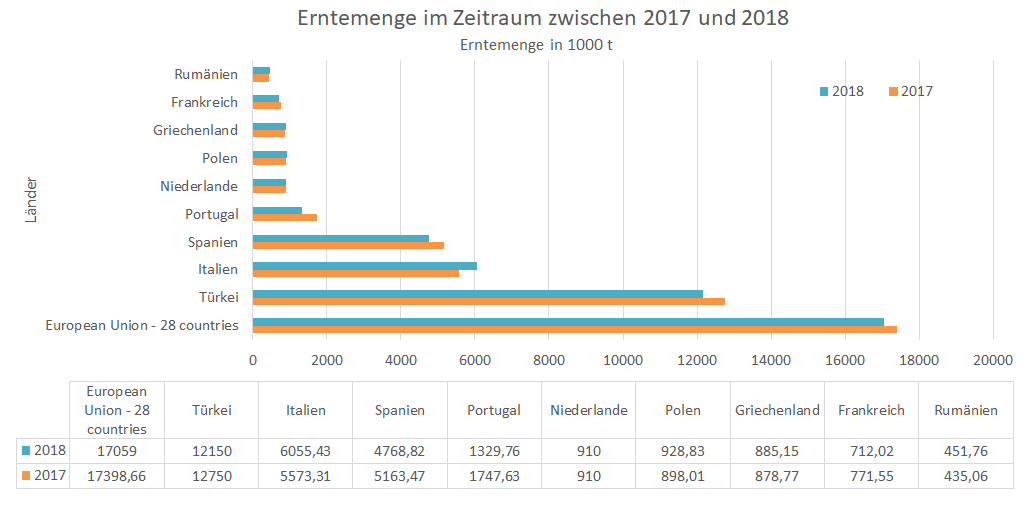
\includegraphics[width=0.9\textwidth]{bilder/erntemenge.PNG}
	\caption{Darstellung der Erntemenge\cite{eurostat} von europäischen Ländern in dem Zeitraum zwischen 2017 und 2018 (eigene Darstellung).}
	\label{erntemenge}
\end{figure}




\newpage
\section{Blattkrankheiten von Tomaten}
\label{sec:Blattkrankheiten}

Es existieren einige Pflanzenkrankheiten, die die Blätter von Tomaten angreifen können. Hier werden vier, nämlich die Dürrfleckenkrankheit, das TYLCV-Virus, die Samtfleckenkrankheit und die Krautfäule, mit ihren typischen Symptomen und Eigenheiten vorgestellt. 


\subsection{Dürrfleckenkrankheit}

%TODO: Sortieren!!! nicht abgeschlossen, \cite{solani}

Die häufigste Krankheit, welche von dem Pilz Alternaria solani verursacht wird, ist die Dürrfleckenkrankheit\cite{borner}. Diese Krankheit tritt besonders bei Tomaten auf und kann in Regionen, die starke Niederschläge, hohe Luftfeuchtigkeit sowie hohe Temperaturen bei $24^\circ-29^\circ\text{C}$ aufweisen, zu einer vollständigen Entlaubung führen. In überwiegend trockenen Klimazonen mit häufigen und anhaltenden, nächtlichen Tauen können sogar Epidemien auftreten. Des Weiteren greift der Pilz nicht nur die Blätter an, sondern zeigt auch Symptome an den Hauptstämmen der erwachsenen sowie jungen Tomatenpflanzen. Die Frucht selbst kann bei einem Befall faulen\cite{solani}. 


\subsubsection{Krankheitserreger}

Der Pilz Alternaria solani wurde zum ersten Mal von Ellis und Martin im Jahr 1882 als A. porri f. sp. solani beschrieben und gehört zu den Fungi imperfecti (Deuteromycotina) in der Klasse Hyphomycetes und Ordnung Hyphales. Alternaria solani gehört zu der Gruppe der großporigen Pilze, welche durch getrennte Konidien, die eine bestimmte Form von einer Spore ist, gekennzeichnet sind und auf einem einfachen Konidiophor getragen werden. Konidiophore bestehen aus fadenförmigen Zellen. Die Konidien von Alternaria solani sind dunkel und ellipsenförmig (s. Abbildung \ref{konidien}). Des Weiteren hat der Pilz mehrkernige und dunkel gefärbte Zellen. Die dunkle Farbe, die von Melanin gebildet wird, schützt den Pilz vor widrigen Umgebungsbedingungen und Mikroben\cite{solani}.

 
%TODO Bild an der richtigen Stelle bringen
\begin{figure}[h!]
	\centering
	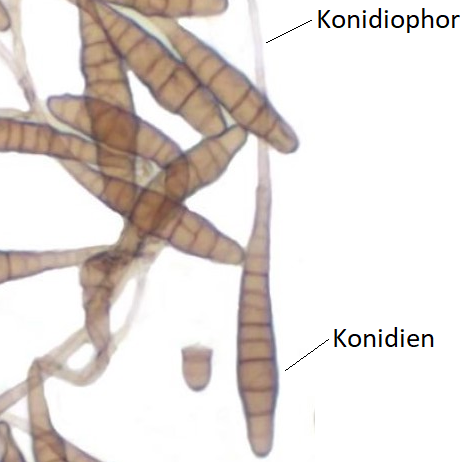
\includegraphics[width=0.7\textwidth]{bilder/konidien.png}
	\caption{In der Abbildung ist zu sehen, wie Konidien vom Erreger Alternaria solani aufgebaut sind. Der Körper des Erregers besteht aus mehreren Konidien in einer Kette gegliedert, welcher mit dem fadenförmigen Konidiophor verbunden ist\cite{konidien}.}
	\label{konidien}
\end{figure}

\subsubsection{Bekämpfung}

Ertragsverluste bis zu 79\% wurden aus Kanada, Indien, Nigeria sowie in den Vereinigten Staaten berichtet. Fäulnisse an dem Stammfuß können zu Verlusten (um die 20 - 40\%) von Keimlingen auf dem Feld führen. Erfolgreiche Bekämpfungsmaßnahmen gegen den Pilz sind beispielsweise Fungizide, die regelmäßig angewendet werden, sowie die Einsetzung von krankheitsfreien Jungpflanzen. Dabei zählt die Behandlung mit Fungiziden zu der wirksamsten Bekämpfungsmaßnahme, die aufgrund der Wirtschaftlichkeit nicht in allen Regionen der Welt durchgeführt wird und bei bestimmten Wetterkonditionen nicht effizient sein könnte. Resistente Sorten sind potenziell die wirtschaftlichste Bekämpfungsmaßnahme, da sie mit Fungiziden kombiniert werden können, um dabei die Kontrolle über den Pilz halten zu können. Allerdings ist die Züchtung von resistenten Pflanzen schwierig, da effektive resistente Gene in kultivierten Tomatenpflanzen kaum vorhanden sind\cite{solani}.

\subsubsection{Krankheitskreislauf}

Die Konidien keimen bei hoher Luftfeuchtigkeit beziehungsweise nahezu gesättigter Feuchtigkeit bei Temperaturen zwischen $8^\circ - 32^\circ\text{C}$ zu einem oder mehreren Keimrohren. Diese dringen anschließend in die Epidermal-Zellen oder durch Wunden aufgrund des Wachstums ein. Das Eindringen benötigt eine gewisse Temperaturspanne, die zwischen $10^\circ$ und $25^\circ\text{C}$ liegt. Die Zellwände des Wirts werden durch Enzyme, hier Cellulase und Pektinmethylgalacturonase, beschädigt, um Toxine abzulassen, die die Wirtszellen abtöten. Dadurch kann der Pilzerreger Nährstoffe aus den toten Zellen beziehen. Verletzungen von einer Infektion sind erst nach zwei bis drei Tagen sichtbar. Des Weiteren erfolgt die Produktion von Sporen ab dem dritten bis fünften Tag. Die Infektion selbst findet in einem sehr kurzen Zeitraum statt, so dass eine polyzyklische Infektion ermöglicht wird. Der Pilz überlebt als Konidien im Boden, in Pflanzenresten und in Samen. Weitere Überlebensmöglichkeiten des Erregers sind beispielsweise Chlamydosporen, welche durch die Zellteilung entstanden sind. Daher umfasst der Lebenszyklus von Alternaria solani den Boden-, Saatgut- und Luftbereich, so dass die Kontrolle des Erregers erheblich erschwert wird. Die Hauptwirte des Erregers sind Pflanzen aus der Familie der Nachtschattengewächse, beispielsweise Tomaten, Kartoffeln, Auberginen und Paprika\cite{solani}.

In der Abbildung \ref{solani_circle} wird der Krankheitszyklus veranschaulicht. Ausgehend von einer Infektion können Konidien in den Pflanzenresten und Samen überleben. Anschließend keimen Konidien, um die Zellwände entweder direkt zu durchdringen oder durch eine Wunde in das Zellinnere einzudringen. Bei dem Eindringen durch die Wunde werden die Früchte oder der Stamm infiziert. Das direkte Eindringen infiziert die Blätter der Pflanze, die Verletzungen auf Blättern, dem Stamm sowie der Frucht auslösen. Ausgehend von dieser Lage können neu produzierte Konidien die Pflanze erneut infizieren.  

\begin{figure}[h!]
	\centering
	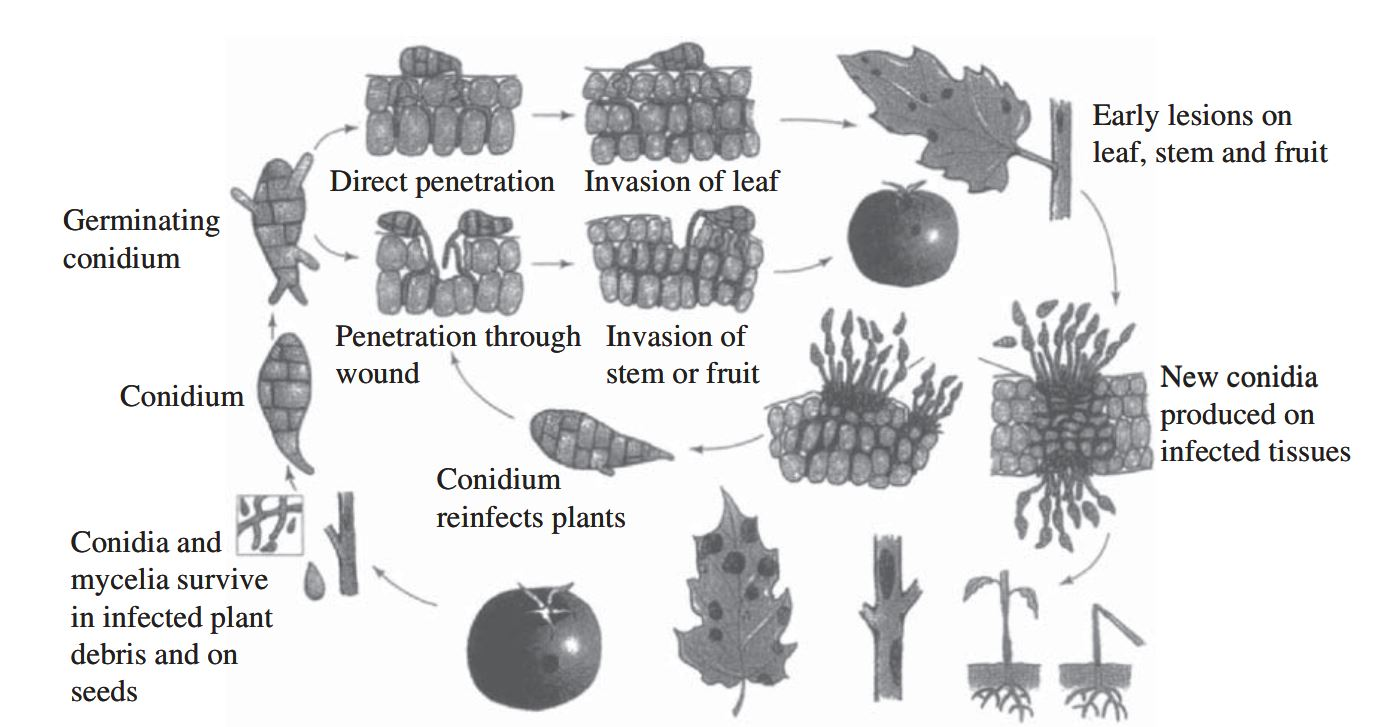
\includegraphics[width=\textwidth]{bilder/solani_circle.jpg}
	\caption{Darstellung des Krankheitskreislaufs mit einer polyzyklischen Struktur\cite{solani}.}
	\label{solani_circle}
\end{figure}


\subsubsection{Krankheitssymptome}

%todo Bild?

Alle oberirdischen Bestandteile der Pflanze können von Alternaria solani befallen werden und zeigen unterschiedliche Symptome an den Blättern, Früchten sowie Stämmen\cite{borner,solani}:

\begin{itemize}
	\item Dürrfleckenkrankheit: Die Symptome von dieser Krankheit bestehen aus kleinen, dunklen, nekrotischen Verletzungen auf den älteren beziehungsweise unteren Blättern. Mit zunehmendem Alter breitet sich die Krankheit zu den oberen Blätter aus. Die Verletzungen haben meist konzentrische Ringstrukturen, die oft von einer Vergilbungszone begleitet werden. Bei einer schweren Infektion sorgt Alternaria solani für ein vorzeitiges Absterben des Laubs, welches die Pflanze schwächt. Wegen der Schwächung können die Früchte durch Sonneneinstrahlungen verletzt werden. 
	 
	\item Fruchtfäule: Bei grünen oder reifen Früchten können am Stielende dunkle, versenkte Stellen auftreten. Der Auslöser dieser Stellen ist eine Stammverletzung, die eine beträchtliche Größe erreichen kann. Grundsätzlich sind halbreife Früchte anfälliger als reife. Des Weiteren fallen stark infizierte Früchte ab, bevor sie die Reifung erreicht haben. 
	
	\item Stammfäule: An den Hauptstielen und Seitenästen von erwachsenen Pflanzen verursacht der Pilz kleine, dunkle, leicht versunkene Stellen, die sich zu dunkelbraunen, länglichen Flecken vergrößern. Diese Vergrößerungen bilden konzentrierte Ringe, die auch auf den Blättern zu finden sind.
	
\end{itemize}




\subsection{Tomato Yellow Leaf Curl Virus}


In vielen tropischen und subtropischen Regionen weltweit stellt das Tomato Yellow Leaf Curl Virus (TYLCV) eine Bedrohung für die Tomatenproduktion dar\cite{TYLCV}. Am Ende der 1930er Jahre wurde von Schäden, die durch diese Krankheit verursacht wurden, berichtet. In Ländern des Nahen Ostens ist der Tomatenanbau von dieser Krankheit seit den 1960er Jahren stark betroffen. Die Ursache der Krankheit ist das Geminivirus, das einen zirkulären DNS-Einstrang hat und durch Insekten verbreitet wird\cite{gemini}. Mittels der weißen Fliege (Bemisia Tabaci), die als Vektor für diese Krankheit dient, wird diese Krankheit übertragen. Der B-Biotyp von Bemisia Tabaci ist seit den späten 1980er Jahren weltweit verbreitet. Dieser kennzeichnet sich durch ein breiteres Wirtsspektrum im Vergleich zu anderen Biotypen aus, so dass dieser nicht nur Unkraut oder Pflanzen, die geographisch auf ein bestimmtes Gebiet beschränkt sind\cite{endemic}, infiziert, sondern auch benachbarte nicht betroffene Kulturarten. Die TYLCV-Krankheit korreliert in tropischen und subtropischen Regionen in den letzten zehn Jahren mit den Ausbrüchen des B-Biototyps von Bemisia tabaci. Berichte aus dem Mittleren und Nahen Osten, Afrika, Europa und Mittelamerika vermerken Schäden an Tomatenkulturen, die auf die Virusart der TYLCV-Gruppe zurückzuführen sind. Das TYLCV-Virus wurde kürzlich in Japan, Mexiko sowie in Florida und Georgia in den Vereinigten Staaten von Amerika gemeldet. 

\subsubsection{Interaktionen zwischen dem Wirt und dem Virus}


Studien mit TYLCV-Is, TYLCV-Sar und verschiedene Quellen von Bemisia tabaci wurden durchgeführt, um Kenntnisse einer erfolgreichen Übertragung ermitteln zu können. Allerdings ist noch mehr Forschung notwendig, bevor die Mechanismen, die die Wechselwirkungen regeln, vollständig verstanden werden, um die Übertragung von Viren zu verhindern\cite{TYLCV}. 

Die minimale Übertragungszeit des Virus lässt sich in dem Intervall zwischen 17 bis 24 Stunden eingrenzen\cite{TYLCV}. Weibliche Fliegen sind anfälliger für das Virus als männliche und dienen daher vermehrt als Vektoren. Nymphen sind genau so anfällig wie Ausgewachsene, um das Virus zu bekommen. Mit steigendem Alter fällt die Anfälligkeit für eine Übertragung ab. Diese infektiösen weißen Fliegen können das Virus dann zehn bis zwölf Tage lang behalten und während der Nahrungsaufnahme in eine beliebige Anzahl gesunder Tomaten injizieren. Nach diesem Zeitraum müssen die Fliegen das Virus wieder erwerben, indem sie sich von einer infizierten Pflanze ernähren\cite{leaf_curl}. Des Weiteren ist das Virus für die weiße Fliege schädlich, da er auf die Lebenserwartung und Fruchtbarkeit einen Einfluss hat. Vermutlich kann sich das Virus in der Fliege reproduzieren. Allerdings wurde dies nicht bestätigt.


\subsubsection{Symptome}

Das Virus verursacht eine Krankheit, die bis zu einem totalen Gesamtertragsverlust führen kann\cite{leaf_curl}. Ihre Symptome lassen sich folgendermaßen beschreiben (s. Auflistung \ref{yellow_list}). Das Aufwärtsrollen der Blattränder ist das bekannteste Merkmal. Neben der Verkümmerung von Blättern sowie Blütenabstoßungen reduziert sich auch die Blattfläche und junge Blätter vergilben. Falls eine Infektion in frühem Wachstumsstadium vorliegt, dann ist der Verlust des Produktionsertrags fast absolut. Außerdem löst die Infektion den Rückgang des Pflanzenwachstums aus. Des Weiteren sollten bei der visuellen Diagnose von TYLCV mindestens zwei Symptome oder mehr vorliegen, um eine Fehldiagnose ausschließen zu können. Einzelne Symptome, zum Beispiel Blattvergilbung oder Blattkräuselung, können durch spezifische Umwelteinflüsse verursacht werden. 

\begin{itemize}
	\label{yellow_list}
	\item Blattvergilbung: Jüngere Blätter sind von einer Vergilbung des Blattes betroffen.
	
	\item Blattkräuselung: Das nach oben Aufrollen der Blattränder ist ein typisches Merkmal von TYLCV.
	
	\item Verkümmerung: Kombinationen von Viren können die Standfestigkeit der Pflanze reduzieren und eine verkümmelte Pflanze verursachen. 
	
	\item Blütenverlust: Der Verlust der ersten Blüte kann durch Umgebungsbedingungen oder leichte Ungleichgewichte in der Bodenfeuchtigkeit ausgelöst werden. Eine anhaltende Blütentrennung ist ein deutlicher Hinweis auf das TYLCV-Virus.
	
	\item Reduzierte Blattgröße: Neben der Verkümmerung von Blättern sowie Blütenverluste reduziert sich auch die Blattfläche.
\end{itemize}

\subsubsection{Verbreitung}


Für viele der Regionen, in denen das Virus sehr stark verbreitet ist, liegen nur begrenzte Informationen über TYLCV-Epidemien vor. Berichte über die natürliche Verbreitung des TYLCV-Virus auf der Grundlage groß angelegter Umfragen sind jedoch selten. Im Allgemeinen deuten die verfügbaren Daten darauf hin, dass das TYLCV-Virus in Unkrautwirten nicht weit verbreitet ist. In Ländern, zum Beispiel Spanien und Italien, verursacht das TYLCV-Sar Virus seit Ende der 1980er bzw. Anfang der 1990er Jahre schwere Epidemien bei Tomaten. Allerdings wurden nur die einjährigen Unkrautarten, hier D. stramonium, S. nigrum, S. luteum und Euphorbia sp., mit diesem Virus infiziert. Studien in Italien zeigten, dass sich das Auftreten von B. tabaci im Freien auf wärmere Regionen, in denen TYLCV-Epidemien auftreten\cite{TYLCV}, beschränkt. 


\subsection{Samtfleckenkrankheit}

Die Samtfleckenkrankheit tritt in manchen Regionen, zum Beispiel in Neuengland, nur in Gewächshäusern auf und befällt hauptsächlich Tomaten. Für den Ausbruch dieser Krankheit wird eine hohe Luftfeuchtigkeit beziehungsweise feuchte Pflanzenoberfläche benötigt\cite{Greenhouse}.


\subsubsection{Erreger}
Die Samtfleckenkrankheit, die erstmals von Cooke im Jahre 1883 beschrieben wurde \cite{Passalora}, wird von einem Pilzerreger, hier Cladosporium fulvum, verursacht, welcher auch unter dem Namen Passalora fulva beziehungsweise Fulvia fulva bekannt ist\cite{Cladosporium, leaf_mold}. Dieser zeichnet sich dadurch aus, nur Tomaten zu befallen\cite{leaf_mold}. Meistens sind die Blätter das einzige vom Pilz befallene Gewebe, dennoch können gelegentlich auch Stängel, Blüten, Stiele und Früchte befallen werden\cite{Passalora}.


\subsubsection{Symptome}

Von einer Infektion sind die ältesten Blätter zuerst betroffen. An den Oberseiten der Blätter bilden sich hellgrünlich-gelbe Flecken mit keinen ausgeprägten Rändern. Dabei sind die Flecken kleiner als 6,35 mm. Auf der unteren Blattfläche unterhalb der Blattflecken ist ein olivgrüner bis brauner Samtschimmel, zu erkennen (s. Abbildung \ref{samtflecken_bilder}). Des Weiteren können Blattflecken zusammenwachsen. Im weiteren Verlauf der Krankheit fangen die Blätter an, zu welken und zu sterben. Diese Blätter bleiben dennoch oft an der Pflanze hängen. Blüten, die auch infiziert sind, werden schwarz und fallen von der Pflanze ab. Bei einer Fruchtinfektion entstehen glatte, schwarze, unregelmäßige Fläche am Stammende der Frucht, die versenkt, trocken und ledrig werden\cite{Greenhouse, Passalora}. 


\begin{figure}[h!]

	\hfill
	\subfigure{
		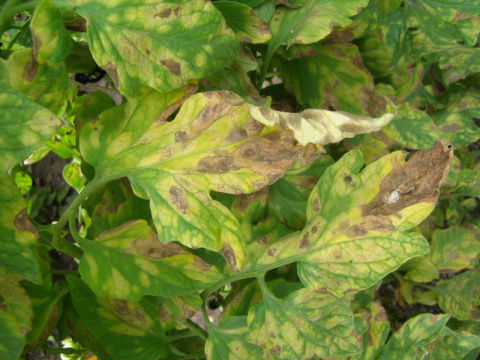
\includegraphics[width=0.45\textwidth]{bilder/upper-leaf-mold-tomato.jpg}}
	\hfill
	\subfigure{
		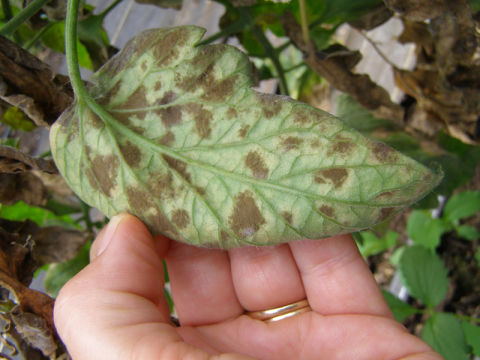
\includegraphics[width=0.45\textwidth]{bilder/leaf-mold-tomato-lower-spores.jpg}}
	\hfill
	\caption{In der linken Abbildung wird die Oberseite mit den hellgrünlich-gelbe Flecken visualisiert. Auf der unteren Seite des Blattes (rechte Abbildung) sind die einzelne Samtschimmelflecken klar zu erkennen\cite{leaf_mold}.}
	\label{samtflecken_bilder}
\end{figure}



\subsubsection{Krankheitsverlauf}

Sporen von dem Erreger können bei Zimmertemperatur auf dem Boden für sechs bis zwölf Monate überleben. Innerhalb der infizierten Pflanzenresten bildet der Erreger dunkle, harte Ruhestrukturen, in diese eine Menge neuer Sporen unter Lufteinwirkung produziert werden können. Durch diesen Mechanismus sichert sich der Erreger das Überleben von einer Jahreszeit zur nächsten. Des Weiteren kann der Erreger mittels Tomatensamen in ein anderes Gebiet eingeschleppt werden, weil er in und auf den Tomatensamen überleben kann.
Der optimale Temperaturbereich für eine Infektion, die von den Sporen ausgelöst wird, liegt zwischen 21$^\circ$ und 23$^\circ\text{C}$. Eine Luftfeuchtigkeit ab 85\% löst eine schwere Samtflecken-Epidemie aus. Dennoch kann diese Krankheit auch bei einer Luftfeuchtigkeit von weniger als 85\% auftreten. Die unteren Blätter der Pflanze sind bei der Infektion zuerst betroffen. Innerhalb eines Zeitraums zwischen zehn bis zwölf Tagen bilden sich neue Sporen auf der Unterseite der infizierten Blätter. Falls die Feuchtigkeit über 85\% bleiben sollte, dann können diese Sporen neue Blätter infizieren. Innerhalb der Anbauphase können mehrere Generationen des Erregers durch die Konidien von Blatt zu Blatt und von Pflanze zu Pflanze aufgrund von Wind, Regen und Insekten weiter verbreitet werden\cite{leaf_mold, Passalora, Greenhouse}.







\subsection{Krautfäule}

Weltweit ist die Krautfäule\cite{rapid_detect} als Erkrankung bei Kartoffeln und Tomaten bekannt. Vor dem Jahr 1992 wurden kaum Epidemien von Krautfäulen in den meisten Teilen der Vereinigten Staaten und Kanadas dokumentiert. Allerdings änderte sich dieser Zustand in den Jahren 1992 und 1993. Dieser Zeitraum zeichnete sich durch schwere Krautfäule sowohl auf Kartoffeln als auch auf Tomaten aus. Seit dem wird über die Krautfäule jährlich berichtet. Des Weiteren hindert die Krankheit in vielen Entwicklungsländern die Ausweitung des Kartoffelanbaus und sorgt jährlich für eine exzessive Anwendung von chemischen Fungiziden, die zu Resistenzen führt.  



\subsubsection{Erreger}
%QUELLE HINZUFÜGEN \cite{lbopat}lbopat hauptquelle


Die erste Entdeckung des Erregers\cite{lbopat} Phytophthora infestans wurde in den 1840er Jahren von M. J. Berkeley dokumentiert. Der Erreger gehört der Gruppe Oomycetes an und wird auch als Wasserschimmelpilz bezeichnet. Der Familienname für diese Gruppe von Organismen ist Peronosporaceae, die der Klasse Stramenopila der Eukaryonten zugeordnet werden. Die Pilze der Gruppierung Oomycetes sind keine echte Pilze, da sie mit den Braunalgen in enger Beziehung stehen. Der Zellkern beinhaltet einen doppelten Chromosomensatz (diploid), welcher für die meisten Pilzarten unüblich ist, da sie einen einfachen Chromosomensatz haben. 

An den Bildungsstätten von Sporen (Sporangien) bilden sich sackartige Strukturen auf den Sporangienträger (Sporangiophore), die für die asexuelle Reproduktion notwendig sind (s. Abbildung \ref{late_sack}). Die Sporangiophoren sind miteinander verbunden und produzieren kontinuierlich Sporangien. Durch diese stielartige Struktur werden Sporangien in der Luft verteilt. Der Erreger Phytophthora infestans gehört zu den wenigen Arten, die an eine solche Luftverteilung angepasst ist. Auch auf benachbarten Felder können Sporangien verteilt werden. Allerdings überleben die Sporangien aufgrund der Austrocknung und Sonneneinstrahlung in der Regel nicht. Falls die Felder unbehandelt sind, kann sich der Erreger dennoch von Feld zu Feld ausbreiten\cite{lbopat}.

\begin{figure}[h!]
	\centering
	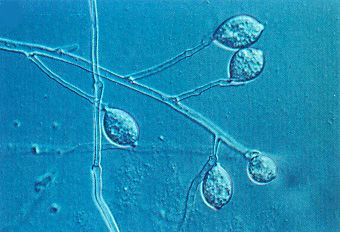
\includegraphics[width=0.7\textwidth]{bilder/LateBlight15.jpg}
	\caption{Darstellung der sackartigen Struktur, die mit dem Sporangienträger (Sporangiophore) verbunden ist\cite{lbopat}.}
	\label{late_sack}
\end{figure}

Unter bestimmten Umweltbedingungen reagieren Sporangien unterschiedlich. Unter wärmeren Bedingungen können Sporangien direkt keimen. Sporangien verhalten sich unter kühlen, nassen Bedingungen jedoch abweichend. Aus den Sporangien treten Zoosporen aus, die zwei Flagellen haben, um auf der Wirtspflanzenoberfläche schwimmen und die Pflanze infizieren zu können\cite{lbopat}.


\subsubsection{Symptome}
%https://cropwatch.unl.edu/potato/late_blights_description hinzufügen da selber inhalt

%\cite{lbopat,CropWatch}
Tomaten sowie Kartoffelpflanzen\cite{lbopat} sind anfällig für die Krautfäule. Die Blattsymptome zwischen Tomaten und Kartoffeln sind ähnlich und weisen nur minimale Unterschiede auf. Die Infektion mit der Krankheit kann wie bei den Kartoffeln schnell erfolgen. Die Bildung von weißen Sporen kann bei feuchtem Wetter erkennbar sein. Des Weiteren kann sich der Erreger in Stängeln sowie Tomatenblättern ausbreiten.

\begin{figure}[h!]
	\centering
	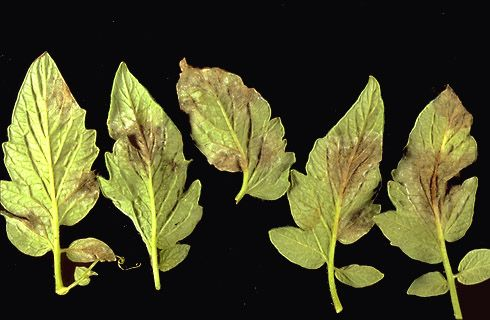
\includegraphics[width=0.7\textwidth]{bilder/LateBlight13.jpg}
	\caption{Infizierte Tomatenblätter weisen typische, dunkelbraune, feste Läsionen auf\cite{lbopat}.}
	\label{lateblight_leaves}
\end{figure}

Die Symptome einer Krautfäule-Infektion kennzeichnen sich durch dunkelbraune, feste Läsionen, die die gesamte Tomatenfrucht zerstören können. Läsionen an den Früchten werden mit leichter Fäulnis und einem Zerfall begleitet. Diese Symptome sind außerdem ähnlich bei den Kartoffeln. Die Abbildung \ref{lateblight_leaves} zeigt solche dunkelfarbige Verfärbungen auf den Blättern von Tomaten. 


\subsubsection{Krankheitskreislauf}

Der Erreger Phytophthora infestans überlebt als Myzel in den Tomatenfrüchten. Falls bei der Ernte infizierte Früchte zurückbleiben, können Sporangien auf den infizierten Früchten entstehen, die im folgenden Frühjahr die Krankheiten auslöst. Durch die Luftströmungen werden die Sporangien zu gesundem Blattlaub getragen und infizieren die Pflanzen. Frisch geschnittene Oberflächen sind besonders anfällig für Infektionen durch luftgetragene Sporen. Wenn ein infiziertes Saatgut gepflanzt wird, kann es zu einer lokalen Infektion kommen. Der Erreger breitet sich durch Bewegung in infiziertem Gewebe aus und die Vermehrung wird durch die asexuelle Reproduktion realisiert.

Außerdem können Sporangien indirekt durch die Produktion und Freisetzung von Zoosporen in Gegenwart von Wasser und bei kühleren Temperaturen keimen. Die direkte Keimung findet bei wärmeren Temperaturen statt. Hierbei bilden die Sporangien ein Keimrohr aus, an dem neue Sporangien entstehen. Grundsätzlich können sich die Sporangien durch Wind und Wasser in neue Teile der Pflanze beziehungsweise neue Pflanzen verbreiten\cite{lbopat}.%\cite{lateblightoverview, lbopat}

In der Abbildung \ref{diseasecircle_late} ist der Krankheitskreislauf veranschaulicht. Ausgehend von einer infizierten Pflanze befinden sich Sporen auf den Blättern, die in der Lage sind, Zoosporen freizusetzen und sich zu verteilen. Somit können weitere Pflanzen infiziert werden. Im Frühling können junge Pflanzen noch Sporen haben, die wiederum auch Zoosporen produzieren, um neue Pflanzen infizieren zu können.

\begin{figure}[h!]
	\centering
	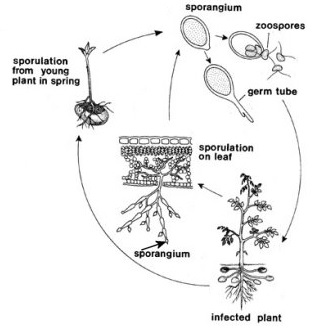
\includegraphics[width=0.7\textwidth]{bilder/LateBlightdiscycle_sm.jpg}
	\caption{Darstellung des Krankheitskreislaufs von der Krautfäule\cite{lbopat} (abgeändert).}
	\label{diseasecircle_late}
\end{figure}

\subsubsection{Verbreitung}
%\cite{lateblightoverview, lbopat}
Die wichtigsten Umweltfaktoren\cite{lbopat} bezüglich der Entwicklung von Krautfäule sind Temperatur sowie Feuchtigkeit und haben einen erheblichen Einfluss auf die Ausbreitung. Falls die relative Luftfeuchtigkeit unter 90\% liegt, dann bilden sich Sporangien auf den unteren Blattflächen und infizieren die Stängeln. Sporangien und Sporangiophore können bei Temperaturen um 3$^\circ$ bis 26$^\circ\text{C}$ auftreten. Der ideale Temperaturpunkt liegt bei 18$^\circ$ bis 22$^\circ\text{C}$. Zwischen 21$^\circ$ bis 26$^\circ\text{C}$ keimen Sporangien mittels eines Keimschlauches. Temperaturen, die unter 18$^\circ\text{C}$ liegen, sorgen dafür, dass Sporangien Zoosporen bilden, die zum Schwimmen Wasser benötigen. Jede einzelne Zoospore kann eine Infektion auslösen. Daher kann die Krankheit bei kühlen, nassen Bedingungen erheblich schwerer ausbrechen. Ganze Felder können bei kühlen Nächten und warmen Tagen unter zwei Wochen zerstört werden, da solche Umweltbedingungen optimal für eine Epidemie sind.



\subsubsection{Bekämpfung}
%\cite{rapid_detect, lateblightoverview}
Aufgrund des hohen Einsatzes von Fungiziden\cite{rapid_detect} sind Resistenzen entstanden, so dass die Einpflanzung von gegen den Erreger resistenten Tomatenpflanzen erheblich erschwert wurde. Infizierte Tomaten lassen sich daher effektiv folgendermaßen bekämpfen\cite{lbopat}:

\begin{itemize}
	\item \textbf{Standortwahl}: Eine gute Entwässerung und Luftzirkulation reduzieren die Luftfeuchtigkeit. Allerdings dürfen Felder, die von Bäumen und einer dichten Vegetation begrenzt werden, nicht benutzt werden. 
	
	\item \textbf{Fruchtfolge}: Zur Bekämpfung der Krautfäule können Rotationen des Feldes von zwei bis drei Jahren stattfinden. Hierbei werden Kulturen verwendet, die für den Erreger nicht als Wirt geeignet sind. Des Weiteren werden nicht nur Kartoffeln und Tomaten von dem Erreger infiziert, sondern auch weitere Nachtschattengewächse.
\end{itemize}

In der Quelle\cite{lbopat} sind weitere Bekämpfungsmaßnahmen bezüglich der Bekämpfung bei Kartoffeln aufgelistet.


